\documentclass{article}


%%PACOTES UTILIZADOS
\usepackage[portuguese]{babel}
\usepackage[a4paper,top=2cm,bottom=2cm,left=2cm,right=2cm]{geometry}
\usepackage{seqsplit}
\usepackage{graphicx}
\usepackage{multicol}
\usepackage{float}
\usepackage{xfrac}
\usepackage{xcolor}
\usepackage{amsfonts}
\usepackage{textcomp}
\usepackage{ascii}
\usepackage{amsmath}
\usepackage{tikz}
\usepackage{setspace}
\usepackage[utf8]{inputenc}
\usepackage{subfig} 
\usepackage{url}
\usepackage{caption}
\usepackage{listings}
\usepackage{minted}
\usepackage{parskip}
\usepackage[colorlinks=true, allcolors=blue]{hyperref}
\definecolor{codegreen}{rgb}{0,0.6,0}
\lstset{
  basicstyle=\ttfamily,
  commentstyle=\color{red},
  keywordstyle=\color{blue},
  upquote=true
}

\linespread{1.25}
    
\setlength{\columnsep}{1cm}

\title{Sequenciamento genético por grafos

MAC0323 EP03 - 2023}


\author{ Matheus Oliveira da Silva - NUSP 13696262 }

\begin{document}
\date{}
\maketitle

\begin{multicols}{2}
\section{Introdução}

O objetivo deste artigo é relatar os resultados e observações das simulações de sequenciamento genético.
O problema de sequenciamento genético é a falta de poder computacional para processar a sequência de grande extensão de uma só vez.

Para tratar tal problema, é aplicado um vírus biológico que quebra a sequência em diversos pedaços pequenos - conhecido como método 'shotgun' - e a partir desses pedaços a sequência original é reconstruída.
Nessa simulação a sequência original é conhecida para fins de testes de eficiência do algoritmo.

Uma série de funções repartirá a sequência original em diversos pedaços, a partir de parâmetros definidos pelo usuário. Após obter todos os pedaços, um grafo é montado com cada pedaço e usando um parâmetro K - que define o tamanho (em número de letras) da ligação os arcos são criados entre os vértices.

É dito que uma aproximação da sequência original será obtida pelo maior caminho, considerando que o grafo não possui ciclos, entre os vértices.

\section{Desenvolvimento}
A maioria das funções foram adaptadas do livro Algorithms\cite{SEDGEWICK}.
\subsection{dna.cpp}
Os parâmetros utilizados nas funções presentes neste arquivo são:

1) string sequence - é a string contendo toda a sequência original que pretendemos aproximar;

2) int N - é o número de pedaços em que a string será repartida;

3) int B - é o tamanho mínimo de cada pedaço;

4) int E - é o tamanho máximo de cada pedaço.

A função random é capaz de gerar números aleatórios em um intervalo fechado.

A função splitdna gera dois números aleatórios para separar a sequência original em N pedaços.

Primeiro o $psize \in [B, E]$, representa o tamanho do pedaço que será construído neste laço;
Segundo o $index \in [0, maxIndex]$, sendo $maxIndex = sequence.size() - psize$ - representando o tamanho máximo que o indíce pode assumir para não extrapolar o tamanho da sequência - e $index$ sendo o índice a partir do qual o pedaço será gerado.

Então o pedaço é uma substring de início $index$ e fim $index + pszie$.
Tal processo é repetido até obtermos N pedaços em um vetor. Por obrigatoriamente N pedaços serem criados, se a sequência não for grande o suficiente, alguns pedaços iguais serão gerados.

Esse processo do projeto simula a quebra da sequência original pelo vírus biológico.

\subsection{createedges.cpp}

Obtendo a lista com todos os pedaços da sequência original, deve ser criado um arquivo para a construção dos arcos que ligarão os vértices que representam tais pedaços.

A condição de ligação entre os vértices é a seguinte:

Se o sufixo do vértice u possui $edgeParam$ ou mais letras iguais ao prefixo vértice v, haverá uma ligação u-$>$v
Os parâmetros utilizados para a criação dos arcos são:

1) vector$<$string$>$ pieces - é o vetor de pedaços gerados pela função $splitdna$;

2) int edgeParam - parâmetro importante que define o número mínimo de letras que devem coincidir entre sufixo de u e o prefixo de v para haver a ligação u-$>$v.

Utilizando as funções:

1) $lower$, que retorna o menor tamanho entre duas strings, é usada para definir o intervalo de comparação entre duas strings no momento de definir se há ou não ligação entre os dois pedaços.

2) $match$, utiliza a função $lower$ e verifica se há um sufixo de u, de tamanho $>= edgeParam$, igual ao prefixo de v, de tamanho igual ao de u. Retorna um valor booleano para a verificação.

A função $createfile$ adiciona as ligações à um arquivo de texto "edges.txt" no formato:

pedaço1 pedaço2

pedaço1 pedaço37

pedaçoN pedaçoX

Indicando que há uma ligação entre o pedaço da esquerda em sentido ao da direita.


\subsection{Digraph.cpp}
O grafo utilizado para a simulação é o grafo direcionado (ou orientado), represetando por uma lista de adjacência.

O espaço ocupado pelo vetor de listas de adjacência é proporcional ao número de vértices e arcos do grafo, ou seja, proporcional ao tamanho do grafo. Portanto, listas de adjacência são uma maneira econômica de representação. Para grafos esparsos, listas de adjacência ocupam menos espaço que uma matriz de adjacências. Sendo o número de vértices V e o número de arcos E. No problema do sequenciamento genético o número de arcos é da ordem $O(V)$, definindo um grafo esparso. O número de arcos somente seria da ordem $O(V²)$ se para cada existisse V arcos saindo de cada vértice, sendo improvável tal feito considerando que teria que ser gerado N vértices iguais.\cite{feofiloff_graphdatastructs}

\subsubsection{Implementação}
A implementação do grafo direcionado, utilizando lista de adjacência, mantem um vetor indexado de vértices associados com uma lista de adjacência.

Algumas funções não triviais são extremamente necessárias para a simulação do sequenciamento genético. Sendo elas:

1) $isEdgeInCircuit$ - recebe dois índices, int u e int v, representando o vértice de origem e o vértice de destino do arco respectivamente. Aplica um algoritmo de busca por profundidade para encontrar um caminho de v para u, caso encontre um caminho retorna true, indicando que o arco está em um circuito, retorna false caso o contrário. Essa função é importante para transformar o digrafo em um digrafo acíclico (DAG), basta aplicar uma remoção de arco para cada arco que estiver em um circuito, lembrando que a ordem de remoção destes arcos afeta o resultado final.

2) $topologicalSortUtil$ - Essa função auxiliar implementa o processo de ordenação topológica em um grafo direcionado acíclico (DAG). Ela recebe um vértice 'v' como entrada, marca o vértice como visitado e, em seguida, realiza uma chamada recursiva para todos os vizinhos não visitados do vértice. O algoritmo continua explorando recursivamente os vizinhos até atingir um vértice sem vizinhos não visitados, momento em que o vértice é empilhado na estrutura de dados 'Stack'. Essa recursão é responsável por definir a ordem de visitação dos vértices no grafo, garantindo que vértices predecessores sejam visitados antes dos vértices sucessores. No final do processo, a pilha 'Stack' contém a ordenação topológica dos vértices do DAG. Esse método é crucial na função principal que busca o caminho mais longo, pois permite determinar a ordem correta de processamento dos vértices, otimizando o cálculo das distâncias e a identificação do caminho mais longo.

3) $longestPath$ - É a função que retorna o resultado final do sequenciamento genético (em int). A função implementa um algoritmo eficiente para encontrar o caminho mais longo em um grafo direcionado acíclico (DAG). O método combina a ordenação topológica com a programação dinâmica, que calcula as distâncias dos vértices a partir do vértice de origem. Inicialmente, os vértices são ordenados topologicamente. Em seguida, o algoritmo atualiza as distâncias dos vértices adjacentes usando a técnica de relaxamento, onde a distância de um vértice é atualizada se for encontrada uma rota mais longa. Ao final, é encontrado o vértice com a maior distância e é reconstruído o caminho mais longo, utilizando o vetor de predecessores. Esse algoritmo é eficiente, pois a ordenação topológica evita o processamento desnecessário de vértices e o uso da programação dinâmica garante que as distâncias sejam calculadas de maneira otimizada.

\subsection{SymbolGraph.cpp}
A classe SymbolGraph é responsável por construir um grafo a partir de um arquivo de entrada contendo símbolos. Ela implementa funcionalidades para criar um índice de símbolos, associando cada símbolo a um índice único, e construir o grafo usando esses índices como vértices.
Assim, podemos manipular o grafo utilizando índices numéricos e, quando necessário, mapear os índices para os seus valores em caracteres.

Portanto, somente na criação dos vértices e na exibição do resultado é necessário o uso dos valores em caracteres dos vértices.

\section{main.cpp}
A função principal irá ser responsável pela definição dos parâmetros e aplicação das classes e funções auxiliares. Os parâmetros de entrada são:

1) string sequence - É a sequência de DNA original utilizada para testar se a simulação está correta. Para fins de testes, sequências aleatórias podem ser obtidas neste link: \href{http://www.faculty.ucr.edu/~mmaduro/random.htm}{Gerador de Sequências};

2) vector<string> pieces - armazenará os pedaços gerados pela função $splitdna$;

3) int numPieces - número de pedaços que serão gerados a partir da sequência (esta variável só deve existir se considerarmos que o pedaço não consome a sequência, isto é, poderia se gerar mais pedaços da sequência do que o número de letras que ela possui);

4) int minSize - tamanho mínimo de cada pedaço;

5) int maxSize - tamanho máximo de cada pedaço;

6) int edgeParam - parâmetro para realizar a conexão entre os vértices;

7) vector<vector<int>> longestPath - vetor de vetores de inteiros que irá armazenar o maior caminho no grafo.

A ordem de funcionamento do código é:

 1º os pedaços são gerados aleatoriamente a partir da sequência original;
 
 2º o arquivo de texto que transcreve quais são os vértices e suas ligações é criado;
 
 3º o grafo de símbolos e o digrafo é criado utilizando a classe SymbolGraph e todos os vértices e arcos são adicionados;
 
 4º o grafo é tratado para se tornar acíclico, caso não seja;
 
 5º encontra o(s) maior(es) caminho(s) no grafo acíclico;
 
 6º traduz o(s) caminho(s) de int para string e exibe-o(s).

\section{Simulações}
As simulações foram conferidas utilizando o site \href{https://globalvision.co/tools/compare-text/}{Compara textos}, que compara duas entradas de texto.

Coloquei a sequência original na parte esquerda e a sequência obtida na parte direita. Caracteres em vermelho são caracteres que a sequência obtida adicionou mas não deveria, caracteres em vermelho são caracteres faltando na sequência obtida.
Se nenhum caractere estiver colorido no resultado, significa que ambas as entradas são idênticas, situação objetivo do sequenciamento genético.

Os arquivos de texto com a sequência original e o resultado estão presentes junto com o arquivo desse relatório.

\subsection{Simulação 1}

\subsubsection{1)a}
\begin{table}[H]
    \centering
    \caption{Parâmetros escolhidos}
    \begin{tabular}{| c | c |}
        \hline
        \textbf{Variável} & \textbf{Valor} \\
        \hline
        numPieces & 100 \\
        minSize & 60 \\
        maxSize & 70 \\
        edgeParam & 35 \\
        \hline
    \end{tabular}
\end{table}


Resultado: 
\begin{figure}[H]
    \centering
    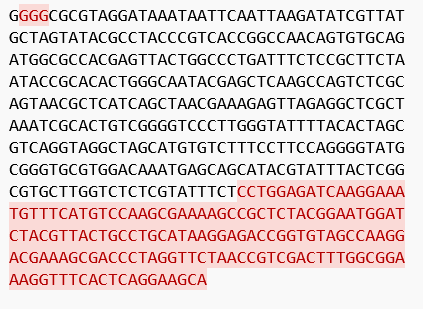
\includegraphics[scale=0.5]{figures/sim1a1.png}
    \caption{}
    \label{sim1a1}
\end{figure}


\subsubsection{1)b}
\begin{table}[H]
    \centering
    \caption{Parâmetros escolhidos}
    \begin{tabular}{| c | c |}
        \hline
        \textbf{Variável} & \textbf{Valor} \\
        \hline
        numPieces & 200 \\
        minSize & 60 \\
        maxSize & 70 \\
        edgeParam & 35 \\
        \hline
    \end{tabular}
\end{table}

Resultado: 
\begin{figure}[H]
    \centering
    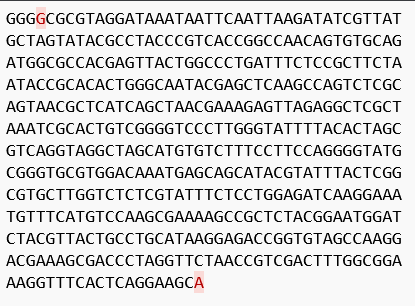
\includegraphics[scale=0.5]{figures/sim1b1.png}
    \caption{}
    \label{sim1b1}
\end{figure}

\subsection{Simulação 2}

\subsubsection{2)a}

\begin{table}[H]
    \centering
    \caption{Parâmetros escolhidos}
    \begin{tabular}{| c | c |}
        \hline
        \textbf{Variável} & \textbf{Valor} \\
        \hline
        numPieces & 100 \\
        minSize & 4 \\
        maxSize & 6 \\
        edgeParam & 2 \\
        \hline
    \end{tabular}
\end{table}

Resultado: 
\begin{figure}[H]
    \centering
    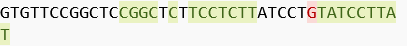
\includegraphics[scale=0.5]{figures/sim2a1.png}
    \caption{}
    \label{sim2a1}
\end{figure}

\subsubsection{2)b}
\begin{table}[H]
    \centering
    \caption{Parâmetros escolhidos}
    \begin{tabular}{| c | c |}
        \hline
        \textbf{Variável} & \textbf{Valor} \\
        \hline
        numPieces & 100 \\
        minSize & 6 \\
        maxSize & 8 \\
        edgeParam & 4 \\
        \hline
    \end{tabular}
\end{table}

Resultado: 
\begin{figure}[H]
    \centering
    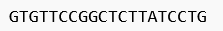
\includegraphics[scale=0.5]{figures/sim2b1.png}
    \caption{}
    \label{sim2b1}
\end{figure}

\subsection{Simulação 3}

\subsubsection{3)a}
\begin{table}[H]
    \centering
    \caption{Parâmetros escolhidos}
    \begin{tabular}{| c | c |}
        \hline
        \textbf{Variável} & \textbf{Valor} \\
        \hline
        numPieces & 500 \\
        minSize & 10 \\
        maxSize & 12 \\
        edgeParam & 6 \\
        \hline
    \end{tabular}
\end{table}

Resultado: 
\begin{figure}[H]
    \centering
    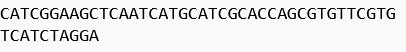
\includegraphics[scale=0.5]{figures/sim3a1.png}
    \caption{}
    \label{sim3a1}
\end{figure}

\subsubsection{3)b}
\begin{table}[H]
    \centering
    \caption{Parâmetros escolhidos}
    \begin{tabular}{| c | c |}
        \hline
        \textbf{Variável} & \textbf{Valor} \\
        \hline
        numPieces & 10 \\
        minSize & 15 \\
        maxSize & 18 \\
        edgeParam & 9 \\
        \hline
    \end{tabular}
\end{table}

Resultado: 
\begin{figure}[H]
    \centering
    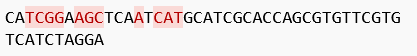
\includegraphics[scale=0.5]{figures/sim3b1.png}
    \caption{}
    \label{sim3b1}
\end{figure}

\section{Conclusão}
A partir da alteração de parâmetros é possível perceber que o $edgeParam$ é um parâmetro extremamente importante, e precisa ser proporcional aos tamanhos dos pedaços, indicando que se bem parametrizado a simulação obtem o resultado correto. Os resultados \ref{sim2b1} e \ref{sim3a1} demonstram que $edgeParam$ sendo a metade de $maxSize$ é uma boa parametrização.

Os testes \ref{sim1a1} e \ref{sim1b1} demonstram que para uma sequência muito extensa, é mais importante a quebra em pedaços grandes do que a quebra em muitos pedaços.

É possível obter uma ótima aproximação, se não perfeita, da sequência original se houver cuidado na parametrização.

\bibliographystyle{plain}
\bibliography{sample}

\end{document}